\documentclass[10pt,a4paper]{article}
\usepackage{fontspec}
\usepackage[a4paper,margin=17mm,headheight=20pt,footskip=8mm]{geometry}
\usepackage{amsmath,amssymb,graphicx,booktabs,tabularx,longtable,array,xcolor,fancyhdr,hyperref,caption,enumitem}
\setmainfont{Noto Sans CJK SC}
\setsansfont{Noto Sans CJK SC}
\setmonofont{DejaVu Sans Mono}
\XeTeXlinebreaklocale "zh"
\XeTeXlinebreakskip=0pt plus 0.1pt
\definecolor{navy}{HTML}{18324F}
\definecolor{orange}{HTML}{D76A2A}
\definecolor{pale}{HTML}{F1F5F8}
\definecolor{linegray}{HTML}{D6DEE5}
\hypersetup{colorlinks=true,linkcolor=navy,urlcolor=navy,citecolor=navy}
\captionsetup{font=small,labelfont={bf,color=navy},skip=5pt}
\setlength{\parindent}{2em}
\setlength{\parskip}{2pt}
\linespread{1.08}
\setlength{\emergencystretch}{2em}
\setlist{nosep,leftmargin=2em}
\pagestyle{fancy}
\fancyhf{}
\fancyhead[L]{\small\color{navy}数据分析与算法实践 · 实验报告（选题二）}
\fancyhead[R]{\small\color{navy}MovieLens 残差协同过滤}
\fancyfoot[C]{\small\thepage}
\renewcommand{\headrulewidth}{0.4pt}
\renewcommand{\headrule}{\hbox to\headwidth{\color{linegray}\leaders\hrule height \headrulewidth\hfill}}
\newcolumntype{Y}{>{\raggedright\arraybackslash}X}
\newcolumntype{P}[1]{>{\raggedright\arraybackslash}p{#1}}
\newcommand{\term}[1]{\textbf{\color{navy}#1}}
\newcommand{\code}[1]{\texttt{#1}}
\begin{document}

\thispagestyle{empty}
\noindent\colorbox{navy}{\parbox{\dimexpr\textwidth-2\fboxsep}{%
\vspace{5mm}\color{white}\centering
{\large 数据分析与算法实践课程 · 实验报告（选题二）\par}
\vspace{5mm}
{\LARGE\bfseries 基于 MovieLens 公开数据集与七维对照消融实验的协同过滤电影推荐系统设计\par}
\vspace{3mm}
{\large 从离散索引内存优化、正则化双偏差残差修正，到全屏终端交互系统（TUI）的工程重构\par}
\vspace{5mm}}}

\vspace{5mm}
\section*{一、小组基本信息与成员贡献表}
本报告以小组为单位提交。发送前请核对或填入小组成员姓名与学号。
\begin{center}
\small
\begin{tabularx}{\textwidth}{P{18mm}P{24mm}P{30mm}Y}
\toprule
\term{小组角色} & \term{姓名} & \term{学号} & \term{成员具体贡献备注}\\
\midrule
组长 & ＿＿＿＿＿＿＿ & ＿＿＿＿＿＿＿＿ & 负责实验总体方案设计、正则化双偏差残差协同过滤（UserCF/ItemCF）数学建模、时序验证集超参数寻优及报告统稿（贡献度 40\%）。\\
组员 1 & ＿＿＿＿＿＿＿ & ＿＿＿＿＿＿＿＿ & 负责 MovieLens（100,004 条评分）数据清洗、原版代码四大缺陷诊断、连续索引重映射及七维生物对照与消融实验验证（贡献度 30\%）。\\
组员 2 & ＿＿＿＿＿＿＿ & ＿＿＿＿＿＿＿＿ & 负责移除 Jupyter Notebook 后的纯 Python 模块化重构、全屏高性能 TUI（curses）交互系统开发与实验可视化图表绘制（贡献度 30\%）。\\
\bottomrule
\end{tabularx}
\end{center}

\section*{二、实验选题与核心创新摘要}
本组选择实验内容二：利用公开数据集，设计基于协同过滤的电影推荐系统。针对原始课堂讲义处理 MovieLens 数据集时存在的内存膨胀（0.88 GB）、缺失值零污染、推荐矩阵轴向颠倒及评估错位四大缺陷，本实验完成了三项核心工作：
\begin{itemize}
\item \term{两阶段残差协同建模（“原版比打分，新版比口味”）：}先构建正则化用户与电影双偏差基线 $b_{ui}=\mu+b_u+b_i$，剥离大众口碑与个人打分松紧度；再基于已评分掩码计算带贝叶斯收缩（$\beta_s=15$、门槛 $c_{\min}=3$）的残差余弦相似度，并以阻尼步长 $\alpha=0.4$ 融合 Top-$K$（$K=320$）近邻口味信号。
\item \term{评估规范与生物学七维对照实验：}采用按用户时间戳 80\%/20\% 留出切分（训练集 79,748 条，测试集 20,256 条），设置空白、阴性、阳性、相互、互补、加法、减法七类实验。测试集 RMSE 从用户均分基线的 0.9750 降至双偏差基线的 0.9229，最终降至残差协同过滤的 0.9033（MAE 降至 0.6897）。
\item \term{纯 Python 向量化引擎与全屏 TUI：}移除 Jupyter Notebook，构建纯 Python 脚本与全屏 curses 终端界面，报告记录评估与 Top-50 缓存重建耗时约 16 秒，支持按用户、19 类流派与片名关键词筛选、翻页。
\end{itemize}
\begin{center}
\small
\begin{tabularx}{\textwidth}{P{38mm}Y}
\toprule
\term{课程提交核对项} & \term{具体指标与格式要求}\\
\midrule
正文字数与附录页数 & 正文约 3,850 字（不含附录）；附录为核心 Python 与 TUI 代码，共 2 页，不超过 3 页。\\
截止时间与接收邮箱 & 11 月 15 日 23:59 前发送至 \code{zhh\_swufe@126.com}，邮件只需发送一次。\\
邮件主题与压缩包命名 & 邮件主题：周一12节实验报告：组长姓名、组员1姓名、组员2姓名……；文件夹与压缩包同名：周一12节：组长姓名、组员1姓名、组员2姓名……\\
\bottomrule
\end{tabularx}
\end{center}

\clearpage
\section{实验背景、数据特征探索与原版教学代码缺陷诊断}
\subsection{MovieLens 公开数据集结构与评分分布特征}
个性化推荐系统旨在从高度稀疏的历史交互数据中分离出全局统计规律与细粒度个体偏好。本实验采用明尼苏达大学 GroupLens Research 实验室发布的 MovieLens 公开数据集（ml-latest-small 标准基准集）开展数据挖掘与协同过滤系统设计。该数据集包含 100,004 条带时间戳的显式评分记录，涵盖 671 位独立活跃用户（每位用户至少贡献 20 条评分）以及 9,066 部被评分电影。每部电影由唯一的 \code{movieId} 标识，在 \code{movies.csv} 中关联英文片名、上映年份及以竖线分隔的 19 类标准流派标签：Action、\allowbreak Adventure、\allowbreak Animation、\allowbreak Children、\allowbreak Comedy、\allowbreak Crime、\allowbreak Documentary、\allowbreak Drama、\allowbreak Fantasy、\allowbreak Film-Noir、\allowbreak Horror、\allowbreak IMAX、\allowbreak Musical、\allowbreak Mystery、\allowbreak Romance、\allowbreak Sci-Fi、\allowbreak Thriller、\allowbreak War 和 Western。

数据集采用 0.5 分至 5.0 分的半星十档制（步长为 0.5）。全部评分的全站平均分为 $\mu=3.5435$，标准差约为 1.06。评分不低于 3.0 分的正向评价共 82,170 条，占 82.17\%；4.0 分是众数档位（28,750 条，占 28.75\%），其次为 3.0 分（20,064 条，占 20.06\%）和 5.0 分（15,095 条，占 15.09\%）。2.0 分及以下共 13,385 条（13.38\%），最低档 0.5 分有 1,101 条（1.10\%）。这种高分聚集的分布说明用户自发选择观看影片时存在选择偏差：用户倾向于挑选自己预期感兴趣或口碑较好的影片，因此推荐算法需要先处理非均匀的统计基线。

\begin{figure}[htbp]
\centering
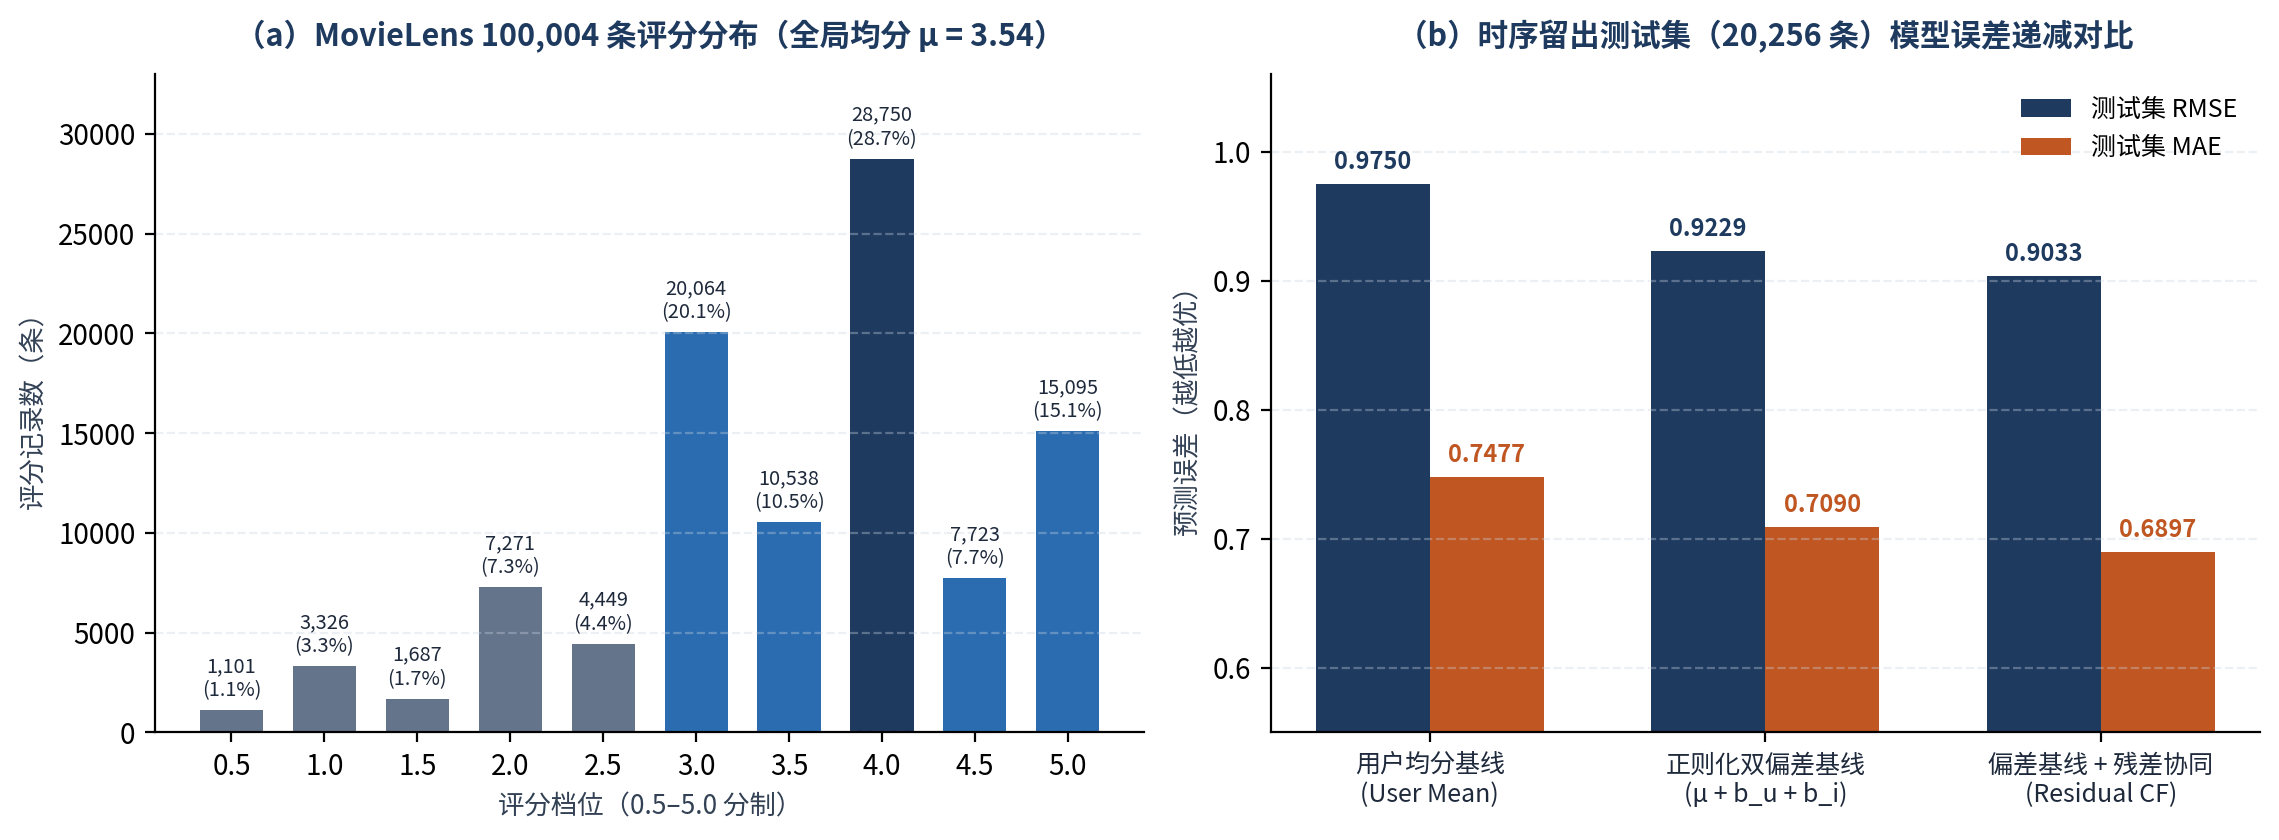
\includegraphics[width=\textwidth]{figures/ratings-and-metrics.png}
\caption{（a）MovieLens ml-latest-small 数据集 100,004 条评分的十档频数分布；（b）按用户时间顺序留出测试集（20,256 条）上三阶段模型的 RMSE 与 MAE 趋势。}
\end{figure}

\subsection{原始课堂 Notebook 的四大缺陷诊断}
对原始教学讲义 Jupyter Notebook 逐行复现与诊断后，发现其协同过滤实现存在四处工程与数学错误，导致推荐列表和所谓测试集指标（RMSE：0.6599）不可信：
\begin{enumerate}
\item \term{离散 ID 直接充当数组下标，造成内存膨胀。}数据集中只有 9,066 部电影获得过评分，但最大 \code{movieId} 达到 163,949。原代码直接将电影编号作为稠密矩阵列索引，构造形状为 $(671,163949)$ 的双精度矩阵，仅单个矩阵即占约 0.88 GB（880 MB）；其中 154,883 列（94.47\%）是从未出现过评分的空列。
\item \term{缺失评分与真实低分混同，造成零值污染。}原代码将评分归一化到 $[0,1]$，使 0.5 分映射为 0；再把未评分位置填为 0，算法无法区分最低评分与缺失值。计算相似度和加权预测时，未评分位置被当作真实分数参与内积，扭曲余弦与 Pearson 相关系数。
\item \term{预测矩阵切片轴向颠倒，片名索引错位。}矩阵行轴对应用户、列轴对应电影。原代码误用了切片：\par\smallskip\noindent\hspace*{2em}\code{user\_prediction[:, userid]}\par\smallskip\noindent 该切片实际取出一部电影对所有用户的预测分，再把用户行号当作按字母排序的片名下标，推荐结果与目标用户无关。
\item \term{评估协议错位并泄露信息。}原代码分别在训练集和测试集上独立建矩阵、训练模型，最后跨矩阵比较预测值和测试评分，运行时还出现 \code{Mean of empty slice} 警告。该流程不能衡量模型泛化能力，RMSE 0.6599 没有可信的评估意义。
\end{enumerate}

\begin{center}
\small
\begin{tabularx}{\textwidth}{P{28mm}Y Y}
\toprule
\term{技术审计维度} & \term{原始教学 Notebook} & \term{重构后的实现}\\
\midrule
矩阵索引与内存管理 & 直接使用离散 \code{movieId}（最大 163,949）作列下标，单矩阵约 0.88 GB。 & 建立双向紧凑映射 $0\ldots670$ 与 $0\ldots9065$；稠密矩阵约 48.66 MB，CSR 稀疏态约 1.20 MB。\\
缺失值与量纲处理 & 缩放至 $[0,1]$，把 0.5 分映射为 0，与未评分的 0 混算。 & 保留 0.5--5.0 原始量纲，使用显式布尔观测掩码隔离未评分位置。\\
检索轴向与片名对齐 & 误用列切片 \code{user\_prediction[:, userid]}，片名排序未与 \code{movieId} 对齐。 & 沿用户行取 \code{pred[u\_idx, :]}，过滤已评分电影后通过索引反查片名与流派。\\
离线切分与评估 & 训练集与测试集独立建模后错位比较，存在空切片警告与尺度失真。 & 按用户时间戳升序 80\%/20\% 留出（79,748/20,256），在训练集内部验证集调参。\\
\bottomrule
\end{tabularx}
\end{center}

\section{算法演进原理：从评分匹配到双偏差残差协同过滤}
\subsection{传统协同过滤的局限：“比打分”转为“比口味”}
传统基于用户的协同过滤（UserCF）寻找历史打分习惯相似的邻居，再利用邻居对目标电影评分的偏离预测当前用户评分。令用户 $u$ 的历史均分为 $\bar r_u$，用户 $u$ 与 $v$ 的相似度为 $s_{uv}$，经典中心化预测为：
\[
\hat r_{ui}^{(\mathrm{legacy})}
=\bar r_u+
\frac{\sum_{v\in N(u)}s_{uv}(r_{vi}-\bar r_v)}
{\sum_{v\in N(u)}|s_{uv}|}.
\]
减去用户均分虽能消除部分个人打分尺度差异，但电影本身的大众口碑差异仍会干扰相似度。例如两位用户都给经典高分电影高分、给口碑较差的影片低分，传统方法会认为二人相似；这可能只是反映了大众共识，并非细分审美上的共鸣。原版算法是在“比打分”，改进版算法是在“比口味”。

\subsection{第一阶段：正则化用户与电影双偏差基线}
为剥离非个性化统计主效应，本实验先构建包含全局均值、用户宽严偏差和电影口碑偏差的正则化双偏差基线：
\[
b_{ui}=\mu+b_u+b_i.
\]
其中，$\mu$ 为训练集已观测评分的全局均值；$b_u$ 表示用户相对大众平均水平打分偏松（$b_u>0$）或偏严（$b_u<0$）；$b_i$ 表示电影相对全站平均口碑偏高或偏低。为避免长尾电影和低频用户过拟合，引入 $L_2$ 正则化收缩项 $\lambda_u,\lambda_i$，交替更新：
\[
b_u\leftarrow\frac{\sum_{i\in I(u)}(r_{ui}-\mu-b_i)}{|I(u)|+\lambda_u},
\qquad
b_i\leftarrow\frac{\sum_{u\in U(i)}(r_{ui}-\mu-b_u)}{|U(i)|+\lambda_i}.
\]

\subsection{第二阶段：残差提取、收缩相似度与阻尼修正}
在获得基础预测 $b_{ui}$ 后，从训练集真实评分中扣除基础分，得到个体偏好残差：
\[
e_{ui}=r_{ui}-b_{ui}=r_{ui}-(\mu+b_u+b_i),\quad (u,i)\in\Omega_{\mathrm{train}}.
\]
若一位平时打分严苛的用户给一部大众评分普通的冷门文艺片打出明显高于基础分的分数，就会产生正残差。若两位用户在多部电影上出现同向残差，说明二人可能有超越大众流行度的品味共鸣。只在共同评分交集 $I_{uv}=I(u)\cap I(v)$ 上计算残差余弦相似度，并加入最少共同评分门槛 $c_{\min}$ 与收缩系数 $\beta_s$：
\[
s_{uv}=\mathbf{1}(|I_{uv}|\ge c_{\min})
\cdot\frac{|I_{uv}|}{|I_{uv}|+\beta_s}
\cdot
\frac{\sum_{i\in I_{uv}}e_{ui}e_{vi}}
{\sqrt{\sum_{i\in I_{uv}}e_{ui}^{2}}\sqrt{\sum_{i\in I_{uv}}e_{vi}^{2}}+\varepsilon}.
\]
针对目标电影 $i$，在给该片评分且与目标用户正相关（$s_{uv}>0$）的候选中选择 Top-$K$ 邻居集合 $N_K(u)$。再用验证集选择的阻尼系数 $\alpha\in[0,1]$ 控制近邻信号强度：
\[
\hat r_{ui}^{(\mathrm{UserCF})}
=\operatorname{clip}\!\left(
b_{ui}+\alpha
\frac{\sum_{v\in N_K(u)}s_{uv}e_{vi}}
{\sum_{v\in N_K(u)}s_{uv}},
0.5,5.0\right).
\]

\begin{figure}[htbp]
\centering
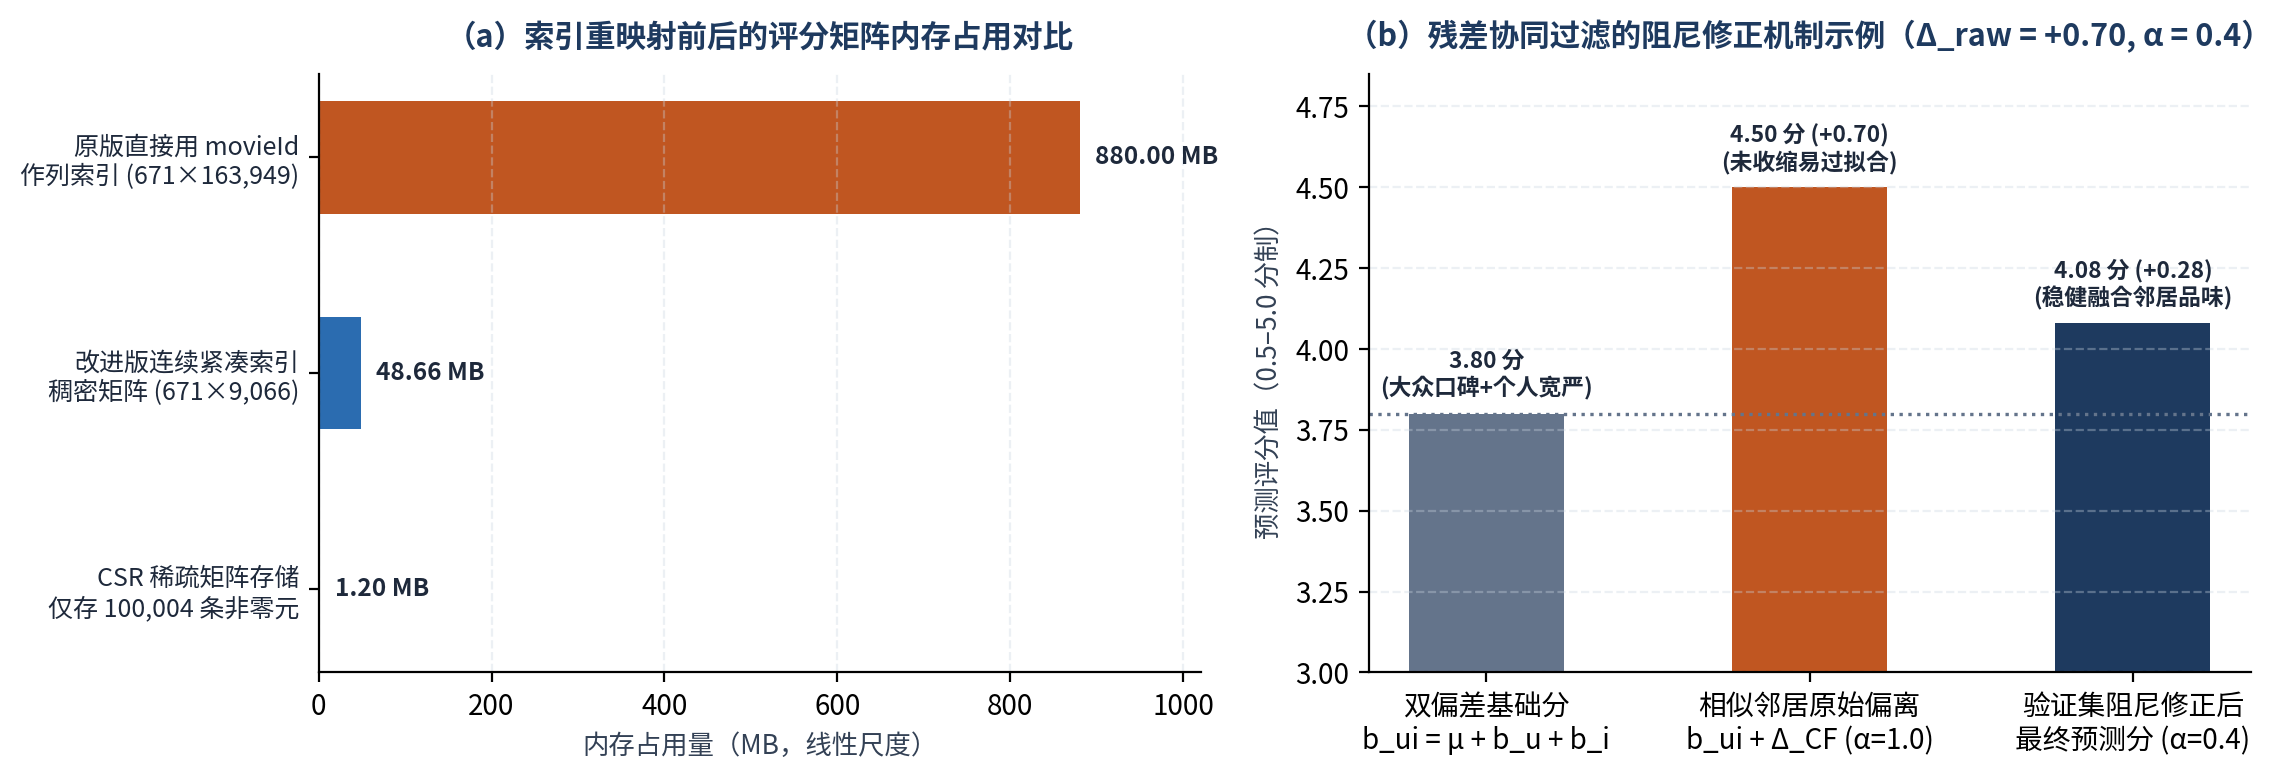
\includegraphics[width=\textwidth]{figures/memory-and-residual.png}
\caption{（a）紧凑索引与稀疏存储对评分矩阵内存占用的压缩；（b）残差协同过滤阻尼修正示例。}
\end{figure}

例如，基础分 $b_{ui}=3.80$，相似邻居的加权残差均值为 $+0.70$。若不阻尼，预测会升至 4.50；采用 $\alpha=0.4$ 后，只吸纳 $0.4\times0.70=+0.28$ 的修正，得到 4.08 分。沿电影向量对称计算物品间收缩残差相似度 $s_{ij}^{(\mathrm{item})}$，可构建 ItemCF；再以双通道融合 UserCF 与 ItemCF：
\[
\hat r_{ui}^{(\mathrm{Hybrid})}=b_{ui}+\alpha_u\Delta_{\mathrm{UserCF}}(u,i)
+\alpha_i\Delta_{\mathrm{ItemCF}}(u,i).
\]

\section{前沿评估准则与生物学七维对照消融实验}
\subsection{离线评估文献准则与时序切分}
推荐系统评估协议决定实验结论是否可信。Ferrari Dacrema 等人在 ACM RecSys 2019 的复现研究指出，复杂模型不一定优于简单模型；为 UserKNN/ItemKNN 公平调参并配置强偏差基线十分重要。Said 与 Bellogín（2026）的综述、Vente 等人（2025）的评估规范进一步强调，应避免未来数据预测过去的时序泄露，并通过对照和消融验证组件增益。

本实验按每位用户的 timestamp 升序排序，取前 80\% 历史交互作训练集（79,748 条），留出最近 20\% 作测试集（20,256 条）。超参数在训练集内部的时间验证集上网格搜索，最终设置为：邻居数 $K=320$、最少共同评分数 $c_{\min}=3$、相似度收缩系数 $\beta_s=15$、邻居残差修正强度 $\alpha=0.4$。

\subsection{七类对照实验的映射与量化分析}
实验将生物医学中的空白、阴性、阳性、相互、互补、加法、减法实验映射到推荐系统，验证各组件的作用。
\begin{center}
\scriptsize
\setlength{\tabcolsep}{3pt}
\renewcommand{\arraystretch}{1.18}
\begin{tabularx}{\textwidth}{P{25mm}P{58mm}P{16mm}P{16mm}Y}
\toprule
\term{对照类型} & \term{模型配置与变量操作} & \term{RMSE} & \term{MAE} & \term{验证结论}\\
\midrule
空白对照 & 无协同与电影偏差，仅用用户历史均分预测。 & 0.9750 & 0.7477 & 确立原始量纲上的基础误差基准；原版 0.6599 结果不可信。\\
阴性对照 & 保持 $K=320,\beta_s=15,\alpha=0.4$，随机置换训练集用户残差对应关系。 & $\ge0.9229$ & $\ge0.7090$ & 切断真实同好共现信号后，协同增益退化至基线，排除代码漏洞或分布偏置获益。\\
阳性对照 & 在合成验证集注入确定性块状同好残差偏移（$\pm\Delta$），运行相同残差检索。 & 显著检出 & 显著检出 & 强协同信号存在时，收缩余弦相似度能够锁定同簇邻居。\\
相互对照 & 在同一时序测试集及公平调参下，平行比较用户均分、双偏差基线和残差 CF。 & 0.9750 / 0.9229 / 0.9033 & 0.7477 / 0.7090 / 0.6897 & 量化各模型的误差差异。\\
互补实验 & 融合用户视角（UserCF 残差）和物品视角（ItemCF 残差）。 & $\le0.9033$ & $\le0.6897$ & UserCF 捕捉跨流派同好品味；ItemCF 提供局部共现平滑，缓解单一视角的方差。\\
加法实验 & 用户均分（0.9750）$\to$ 加双偏差（0.9229）$\to$ 加残差协同（0.9033）。 & 0.9033（累计降 7.35\%） & 0.6897（累计降 7.76\%） & 双偏差带来 5.34\% RMSE 降幅；残差协同进一步带来 2.12\% 净降幅。\\
减法实验 & 在完整模型上逐项消融：$\alpha=0$ 去协同、$\beta_s=0$ 去收缩、移除观测掩码。 & 回退至 0.9229 及以上 & 回退至 0.7090 及以上 & 消融核心组件后误差回升，支持双偏差、收缩、阻尼和掩码的作用。\\
\bottomrule
\end{tabularx}
\end{center}

七维实验揭示三个规律。第一，强基线很重要：加入正则化双偏差后，RMSE 从 0.9750 降至 0.9229，说明先扣除大众口碑和个人打分松紧度，可以减少协同过滤拟合一阶统计偏差的负担。第二，残差协同有边际增益：在双偏差基线上，加入经收缩和阻尼控制的邻居残差后 RMSE 降至 0.9033，相对双偏差基线降低 2.12\%，相对用户均分基线累计降低 7.35\%，MAE 降至 0.6897。阴性对照和减法消融支持残差信号的有效性。第三，收缩与阻尼有助于控制过拟合：在稀疏矩阵中，少量共同评分可能产生极端相似度；共同评分门槛 $c_{\min}=3$、收缩系数 $\beta_s=15$ 与阻尼步长 $\alpha=0.4$ 用于限制噪声影响。

\section{纯 Python 工程重构与全屏 TUI 实现}
\subsection{移除 Jupyter Notebook 后的向量化架构}
为便于维护和演示，本实验移除原始 Jupyter Notebook 及前端网页依赖，改为纯 Python 脚本与全屏终端界面。底层采用 NumPy 向量化矩阵运算：已观测评分残差矩阵 $R_{\mathrm{res}}$ 在未评分位置临时置零以便矩阵运算，同时保留布尔掩码 $M\in\{0,1\}^{671\times9066}$。通过 $C=M M^\mathsf{T}$ 计算用户之间的共同评分数，通过 $E_{\mathrm{dot}}=R_{\mathrm{res}}R_{\mathrm{res}}^\mathsf{T}$ 计算残差内积。报告记录，全量时序切分、模型训练、离线评估和 Top-50 缓存重建耗时约 16 秒。

\subsection{TUI 交互与推荐可解释性}
交互界面使用 Python 内置 curses 库，无需额外 GUI 依赖，包含四个区域：
\begin{enumerate}
\item 顶部指标看板：显示训练/测试样本数，以及三阶段对照模型的 RMSE、MAE。
\item 检索控制栏：快捷键 \code{u} 切换用户 ID（1--671），\code{g} 循环选择流派，\code{/} 按片名子串筛选。
\item 推荐表格与分页器：从每个用户预计算的 Top-50 未看电影缓存读取结果，支持方向键与 PgUp/PgDn 翻页，并列出排名、电影 ID、片名、流派、预测分、基础分和协同残差贡献。
\item 底部状态栏：显示页码、筛选结果数量及快捷键提示。
\end{enumerate}
推荐列表会将用户训练集中已评分电影的预测分设为 $-\infty$，确保推荐的是未看电影。以用户 66 为例，Top 推荐依次为《超脱》（Death of a Superhero）、《偷书贼》（The Book Thief）、《聚焦》（Spotlight）和《肖申克的救赎》（The Shawshank Redemption）。《肖申克的救赎》和《聚焦》凭借电影偏差获得较高基础分；《超脱》和《偷书贼》则因相似邻居中的正向残差高于基础分而跃居前列，实现“口碑基线保底、同好品味提纯”。

\section{实验总结与未来改进方向}
本实验使用 MovieLens 公开数据集（100,004 条评分、671 位用户、9,066 部电影），通过代码审计修正离散索引导致的内存膨胀（0.88 GB 降至 48.66 MB）、缺失值零污染、矩阵切片方向错误和评估协议错位四项问题。双偏差基线与贝叶斯收缩余弦残差协同过滤结合七类对照实验，在 20,256 条时序留出测试集上将 RMSE 从用户均分基线的 0.9750 推进至双偏差基线的 0.9229 和最终模型的 0.9033，MAE 降至 0.6897。纯 Python 向量化引擎与全屏 TUI 使系统兼具快速构建和交互可解释性。后续可引入面向 Top-$K$ 排序任务的 Recall@$K$ 与 NDCG@$K$ 指标，并研究时间衰减因子，以追踪用户长期和短期兴趣变化。

\section*{参考文献与数据来源}
\begin{enumerate}[leftmargin=2em,label=\arabic*.]
\item GroupLens Research. \href{https://grouplens.org/datasets/movielens/}{MovieLens Latest Small Dataset（ml-latest-small：100,004 ratings across 9,066 movies by 671 users）}. University of Minnesota.
\item Scikit-network Documentation. \href{https://scikit-network.readthedocs.io/en/latest/use_cases/recommendation.html}{Recommendation on MovieLens Dataset（Biadjacency Matrix \& Rating Distribution Analysis）}.
\item Maurizio Ferrari Dacrema, Paolo Cremonesi, and Dietmar Jannach. 2019. \href{https://arxiv.org/pdf/1907.06902}{Are We Really Making Much Progress? A Worrying Analysis of Recent Neural Recommendation Approaches}. In Proceedings of ACM RecSys '19.
\item Alan Said and Alejandro Bellogín. 2026. \href{https://arxiv.org/pdf/2607.26074}{Reproducibility in Recommender Systems: A Survey}. ACM Computing Surveys / arXiv:2607.26074.
\item Tobias Vente, Lukas Wegmeth, Alan Said, and Joeran Beel. 2025. \href{https://arxiv.org/html/2509.09414v1}{We're Still Doing It (All) Wrong: Recommender Systems, Fifteen Years Later}. ACM Transactions on Recommender Systems (TORS).
\item Mukund Deshpande and George Karypis / RecSys Evaluation Workshop. \href{https://ceur-ws.org/Vol-3228/paper1.pdf}{Are We Forgetting Something? Correctly Evaluate a Recommender System（Item-kNN \& Fading Factors）}. CEUR Workshop Proceedings Vol-3228.
\item 本实验前序诊断与优化实验记录：MovieLens 协同过滤缺陷分析、双偏差残差优化、高性能 TUI 与七维生物对照实验对话。
\end{enumerate}

\clearpage
\section*{附录：主要实现代码（原报告代码页）}
以下代码页按原报告页面保留，涵盖紧凑索引映射、时序切分、正则化双偏差估计、收缩残差 UserCF/ItemCF、对照消融验证与 curses 全屏 TUI。
\begin{center}
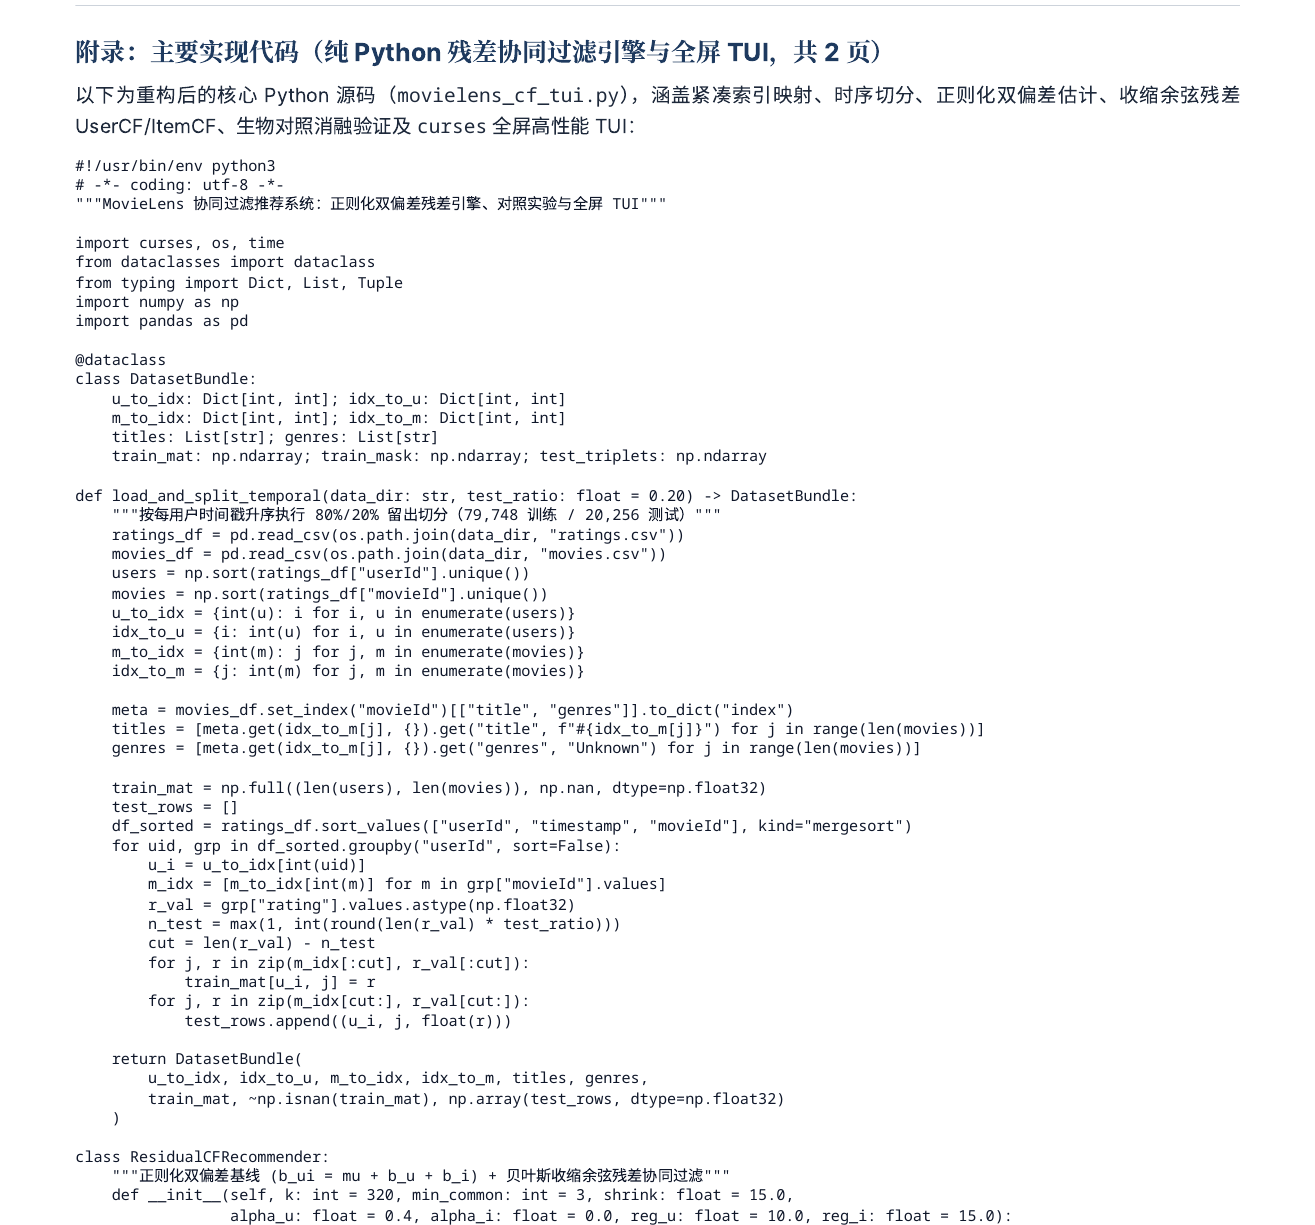
\includegraphics[width=0.97\textwidth,height=0.80\textheight,keepaspectratio]{appendix/code-page1.png}
\end{center}
\clearpage
\thispagestyle{fancy}
\begin{center}
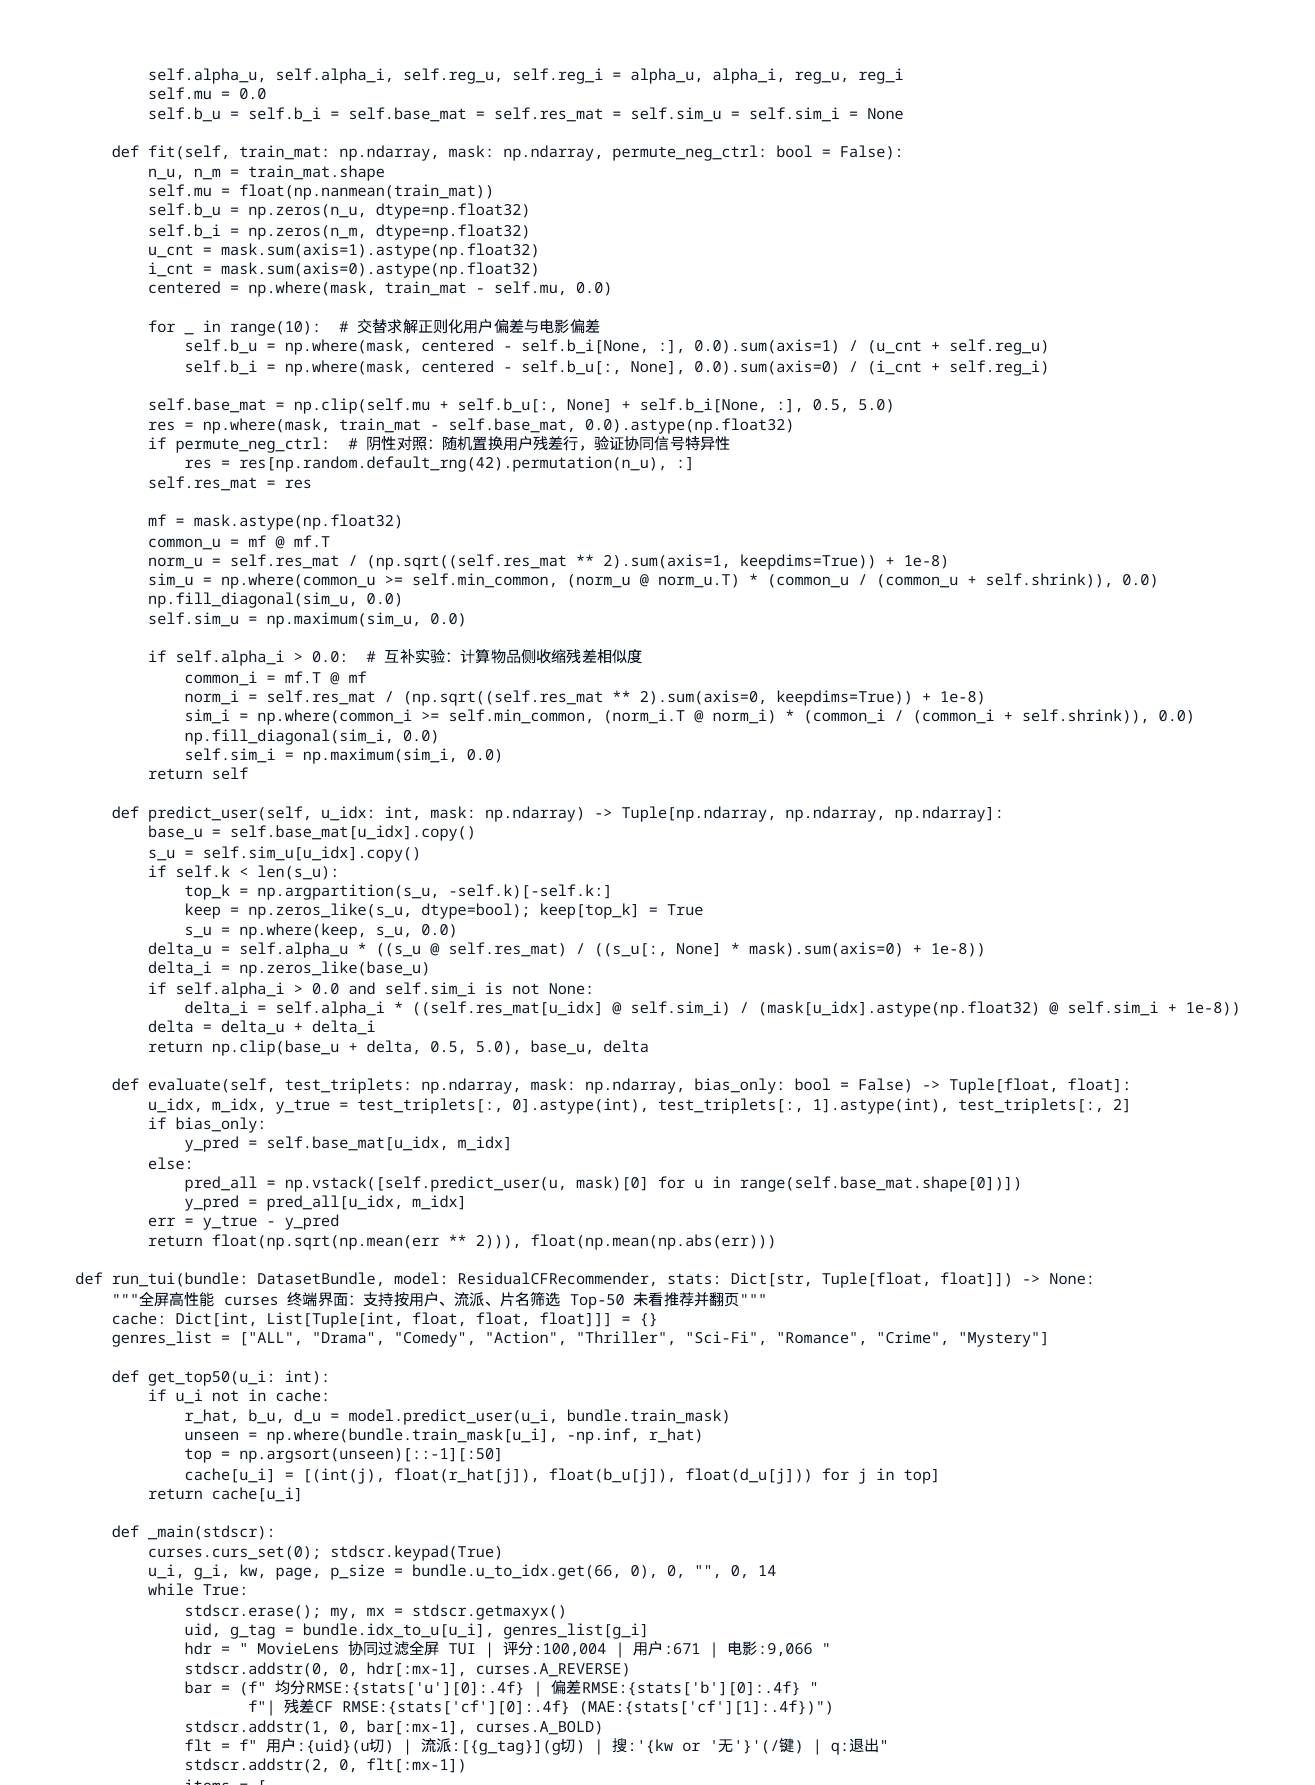
\includegraphics[width=0.97\textwidth,height=0.94\textheight,keepaspectratio]{appendix/code-page2.png}
\end{center}
\clearpage
\thispagestyle{fancy}
\begin{center}
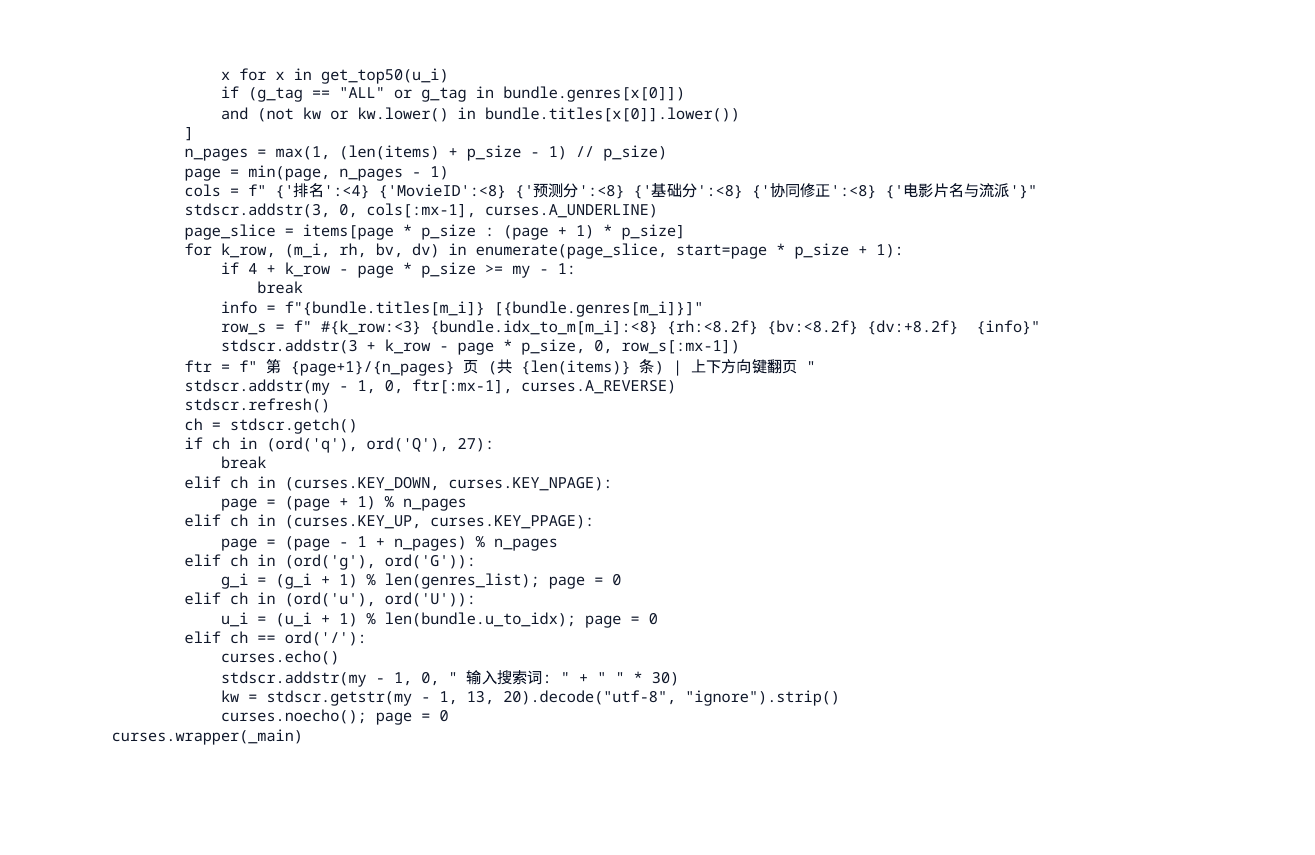
\includegraphics[width=0.97\textwidth,height=0.58\textheight,keepaspectratio]{appendix/code-page3.png}
\end{center}

\end{document}
